% =====================================================================
%  Chapter 1 -- Task Description
% =====================================================================
\section{Task Description}

The goal of this homework project is the modelling of the BME Training Reactor using MCNP, following the benchmark description of the facility~\cite{benchmark}.
A simplified model of the reactor core is built, submerged in a large body of water, and a concrete container is defined around that water as a shield.
The quantity of interest is the neutron dose rate on the outer surface of this concrete container.

The training reactor is characterised by its nominal thermal power of $100~\mathrm{kW}$.
This power fixes the absolute neutron source strength of the core, which is used to scale the simulated, per source neutron, flux into an absolute dose rate at full power.
The model is solved as an MCNP criticality calculation in neutron transport mode.

\begin{figure}[H]
  \centering
  {\setlength{\fboxsep}{0pt}\setlength{\fboxrule}{0.4pt}%
   \fbox{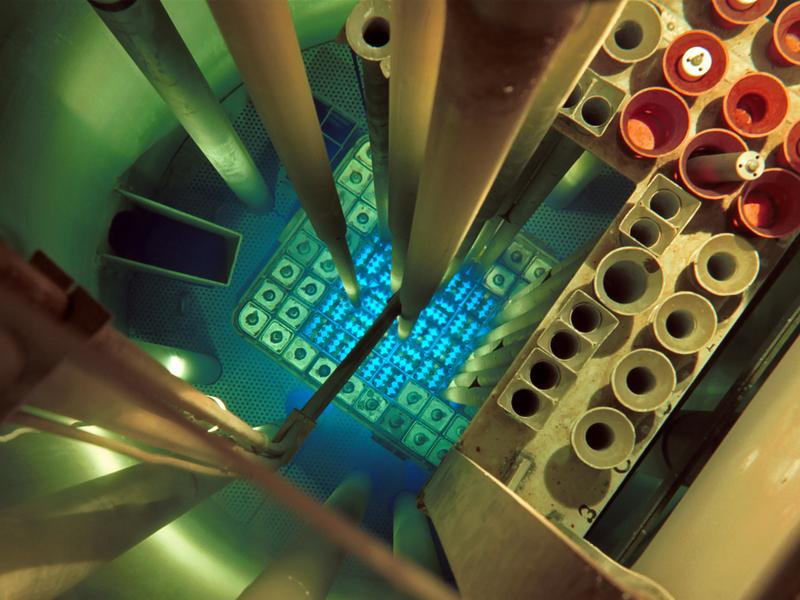
\includegraphics[width=0.8\textwidth]{figures/reactor.jpg}}}
  \caption{Reactor core of the Training Reactor as seen from above.~\cite{benchmark}}
  \label{fig:reactor}
\end{figure}

\newpage
